\documentclass[12pt]{article}
\usepackage[margin=1in]{geometry}
\usepackage{color}   %May be necessary if you want to color links
\usepackage{hyperref}
\usepackage{setspace}
\usepackage{float}
\usepackage{ulem}
\usepackage{bbm}
\usepackage{amsmath}
\usepackage{relsize}
\usepackage{subcaption}
\doublespacing
\hypersetup{
    colorlinks=true, %set true if you want colored links
    linktoc=all,     %set to all if you want both sections and subsections linked
    linkcolor=blue,  %choose some color if you want links to stand out
}
\usepackage{graphicx}
\graphicspath{ {../../images/} }
\setlength{\belowcaptionskip}{-10pt}
\setlength{\abovecaptionskip}{-10pt}
\begin{document}


%g) A thorough description of your methodology.
%h) An explanation and interpretation of your results.
%i) A conclusion summarizing what you’ve done and what it means in a broader context.

%
%a) Title Page - Project title, project adviser, semester, and year.
\begin{titlepage}
	\begin{center}
		\vspace{20pt}
		{\bf \LARGE Indoor Micro-UAV Navigation with Minimal Sensing} \\
		\vspace{200pt}
		Dennis Melamed\footnote{University of Minnesota, Department of Electrical and Computer Engineering}  - 5117411\\
		Advisers: Professor Volkan Isler\footnote{University of Minnesota, Department of Computer Science and Engineering} \& Professor Derya Aksaray\footnote{University of Minnesota, Department of Aerospace Engineering and Mechanics} \\
		Final Report for Senior Honors Design Project (EE 4982V)\\
		Spring 2019 \\
	\end{center}
\end{titlepage}



%a) Title Page - Project title, project adviser, semester, and year.
\begin{titlepage}
	\begin{center}
		\vspace{20pt}
		{\bf \LARGE Indoor Micro-UAV Navigation with Minimal Sensing} \\
		\vspace{200pt}
		Dennis Melamed\\
        \vspace{50pt}
        Submitted under the supervision of Professor Volkan Isler to the University Honors Program at the University of Minnesota-Twin Cities in partial fulfillment of the requirements for the degree of Bachelor Science, summa cum laude in Computer Engineering. \\
        \vspace{50pt}
		\today \\
	\end{center}
\end{titlepage}

\subsection*{Acknowledgments}
I would like to thank Professor Isler and Professor Aksaray for advising this project, Professor Sattar for reading, the members of the RSN lab for their advice, and Ryan Peterson for his help with motion capture systems.



%A 200-300 word abstract clearly summarizing the problem being investigated, why this is an interesting problem, the methodology being used, and the progress to date.
\begin{abstract}
    The usage of a small unmanned aerial vehicle UAV with minimal sensing abilities to navigate complex indoor environments outside a motion capture system has not been well explored. This work develops a system to fly out the door of a room from an arbitrary initial location using a micro-UAV with low-accuracy sensors. The sensing abilities are limited by the payload of the UAV to a low-resolution camera and a low-accuracy IMU. The framework consists of two interacting components: door detection (by a simple Hough transform procedure or a convolutional neural network) and flight control (via proportional-derivative control or a recurrent neural network). The convolutional neural network method for door detection shows significant advantages over the Hough transform-based method in speed and accuracy. The network outperforms the Hough method on both a training dataset and a novel dataset. For flight control, a new payload system for the UAV was built allowing for safe flights and data collection. A ground-truth flight algorithm which used a motion capture system to fly through a door was set up and used for training data collection. The proportional-derivative controller shows success in flying through the door from a fixed location after tuning. Accuracy decreases if the UAV is set in an arbitrary location and the controller is not re-tuned for that location. The recurrent neural network was able to fly the UAV stably but flew in loops without passing through the door. Flying through doors using micro-UAVs on the scale of tens of grams is feasible without an external navigation system by using a convolutional neural network to detect a door and a simple proportional-derivative controller to control flight.
\end{abstract}

%c) Table of Contents - List and page numbers of the different sections.
\tableofcontents

%d) List of Figures - Figure numbers, figure captions, and page numbers.
\listoffigures
\listoftables








%REMOVE FOR 4982 SUBMISSION
%%%%%%%%%%%%%%%%%%%%%%%%%%%%%%%%%%%%%%%%%%%%%%%%%%%%%%%%%%%%%%%%%%%%%%%%5
\section{Non-Technical Summary}
Drones, or Unmanned Aerial Vehicles (UAVs) are a class of robots able to move through the air, often using four propellers giving the name `quadcopters'. Navigating the world is challenging for UAVs, as they do not have the same sensing and processing abilities as humans do. A key task for a UAV is determining where it is in the world in order to navigate to a new, desired location. Many solutions exist for this, including familiar ones such as GPS devices or systems that attempt to replicate human vision in order to track where the robot has moved. Current solutions have drawbacks, including cost, weight, and accuracy. 

Weight and accuracy become significant difficulties as the size of UAVs gets smaller. Smaller UAVs are useful for tasks where a larger UAV may be unable to access the desired space due to its size but where flying through the space is still the best method of completing the tasks. Such tasks might include sewage pipe inspection, agricultural data collection in thick vegetation, and indoor security monitoring. 

In order to complete these tasks, traditionally the UAV has needed to determine where it is in the world, using the previously mentioned localization systems like GPS. This is feasible for larger systems, but very small UAVs cannot lift sensors accurate enough to localize themselves well. This project develops a system where low-quality, lightweight sensors are used on a micro-UAV (27 gram weight) to complete a task which would normally require accurate localization: flying through a door.

To achieve this, two main components are developed. The first is a way to locate where a door is in the low-resolution images available from the micro-UAV's onboard camera. Two different methods of locating the door are created, the first based on more traditional computer vision techniques, the other based on convolutional neural networks, a promising area of network-based image processing that tries to mimic how the human brain processes information. The second major component is a flight controller, which actually tells the micro-UAV where to go based on the location of the door in the current image it sees. Again, two different methods are explored to complete this task. A proportional-derivative controller is a simple system which uses standard control techniques to set the UAV on a course where it will fly through the door. A recurrent neural network uses a network of nodes, again structured to mimic how a brain might deal with information, to get the UAV to fly through the door based on sensor data input. The network learns to do this by being shown hundreds of instances of successful flights and attempts to mimic them. The recurrent neural network also takes advantage of a type of node with memory, which is able to remember past inputs in order to deal with time-dependent quantities like velocities. 

Testing of each implemented method yielded the following results: The convolutional neural network is more accurate and faster than the method based on traditional computer vision techniques. The proportional-derivative controller was more successful at flying the UAV through the door than the recurrent neural network. Neither flight controller was able to achieve a consistently successful flight through the door, but the proportional-derivative controller was able to fly through the door in a small percentage of flights from arbitrary locations.

%%%%%%%%%%%%%%%%%%%%%%%%%%%%%%%%%%%%%%%%%%%%%%%%%%%%%%%%%%%%%%%%%%%%%%%%5









%An introduction summarizing the project and an explanation of its importance.
\section{Introduction}
Most current work in the field of autonomous unmanned aerial vehicles (UAVs) uses well-known localization systems such as GPS, motion capture systems, or onboard sensor fusion to determine the UAV's position and orientation. With this information, control and navigation of the UAV can be achieved through standard algorithms. While these systems are reasonable in certain situations, they each have key drawbacks. GPS devices are heavy and can be inaccurate by several meters depending on the location and model of GPS. Motion capture systems are expensive to install and only allow localization within a small area. Sensor fusion on-board the UAV runs into the same problems as GPS, with accuracy often being relatively poor depending on the environment and sensors used. Weight is an additional concern, as cameras and others sensors sufficient to give good sensor fusion can often weigh more than the payload of the UAV. Due to these issues, it is desirable to find a way a lightweight UAV could move through the world without relying on the above systems to give it its precise location. The applications of such a micro-UAV might include plumbing inspection, agricultural inspection within trees, and indoor security monitoring. This project develops such a platform and creates software for a first step in the complete ability to navigate without the above systems: flying through a doorway. 

Flying through a door is a key task in navigating indoors where a doorway is the most constrained space for a UAV to fly through and thus the most likely place for a crash. The platform selected for this project is a Crazyflie micro-UAV: a low-cost, durable, and open source platform weighing 27 grams. The sensing payload onboard includes an inertial measurement unit (IMU) and a lightweight camera designed for first-person view (FPV) drone racing. Neither of these sensors are very high-quality due to their small size and low cost. While the project task seems simple to a human, a UAV without the ability to completely localize itself must go through several software steps in order to safely fly through the door. 

Detecting a door is the first step. This requires running either a Hough transform-based method or a convolutional neural network on the camera feed coming from the UAV. These methods take in the camera image and output a set of coordinates in the image plane marking where the door is located. Once the door has been localized, the UAV must take off and respond to roll, pitch, yaw, and thrust set points generated by a flight controller. This flight controller must determine which direction to fly in order to make it through the door. Flight control is implemented both as a proportional-derivative (PD) controller and a recurrent neural network (RNN). The PD controller takes as input the location of the door in the image and calculates its distance from the center of the image (directly forward for the UAV). This distance is used as an error term to align the UAV with a path that will lead it through the door. The recurrent neural network approach takes as input the detected door location and other sensor information. Using recurrent layers which are able to remember previous inputs, the network learns to generate the appropriate control inputs for the UAV to pass through the door by mimicking training data. The feasibility of the system and methods described provides a basis for future development of very small-scale systems with limited sensing to complete useful tasks in the real world.

%\begin{figure}
%	\centering
%	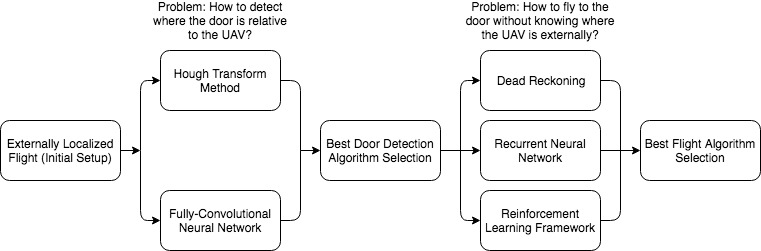
\includegraphics[scale=.55]{flowchart}
%	\vspace{10pt}
%	\caption[Flowchart of Proposed Development Stages]{Flowchart of Proposed Development Stages}
%	\label{flowchart}
%\end{figure}

%A background and summary of previous work in this area, along with an explanation that places the project in the context of what has been done before, and appropriate citations to peer-reviewed sources.
\section{Background}
Previous work in this area falls into a few broad categories. Detection of doors in camera images has been studied in multiple works and is a key initial step in flying through a door. Work in this category includes the detection of elevator doors by JunYoung and Lee \cite{ElevatorDoors} using stereo vision. While the current project will not use stereo vision, the corner detection JunYoung and Lee propose is used in later works. A more relevant publication is Mu\~noz-Salinaz et al.\cite{Fuzzy}, which uses fuzzy logic to successfully detect doors using the edges present in an image including when the door is not completely visible. Tian \cite{Tian2013} attempts to expand on this concept and uses the detection of frame corners and edges to indicate a door, along with the heuristic that doors tend to be inset in the wall while objects similar to doors such as wardrobes tend to extend out from wall. While this is useful for higher resolution cameras, the low accuracy of the camera used in this project makes it unlikely that enough corners and edges are extractable to determine if something is inset or standing out. Llopart, Ravn, and Andersen\cite{NNDoor} use a convolutional neural network to detect doors and cabinets. The network is trained to place a bounding box around any doors in a camera's image. Redmond and Ali \cite{yolov3} develop a fast object detection network called You Only Look Once (YOLO), which places a bounding box around any object class instance it has been trained on. The results of the YOLO work show success and a possible path for development. However, they are unlikely to translate directly to the detection task in this project due to the high resolution and stationary nature of the camera in their work. The low resolution, noisy images generated by the Crazyflie onboard camera require some innovation over the current state-of-the-art detection algorithms. The methods developed here take advantage of problem structure knowledge, such as the fact that the door is unlikely to jump very far from image to image or that doors tend to have certain aspect ratios, in order to improve the accuracy of door detections. 


Indoor navigation of UAVs is a well-researched field. Most research focuses on either UAVs big enough to hold higher-accuracy sensors or systems where the UAV is localized using motion capture setups such as VICON systems. Sanket et al. \cite{gapflyt} makes use of a UAV over ten times the weight of the Crazyflie to detect gaps and fly through them using Temporally Stacked Spatial Parallax, a gap detection method, and a high resolution camera-based approach. Their method is very successful for irregular gaps and proposes the use of a ``safe point'' that is chosen as the location to fly through the gap, calculated to ensure that the UAV will fit through the gap. Riviere, Manecy, and Viollete\cite{Folding} use a micro-UAV shaped like an `H' which is able to fold up to form a narrow body more able to fit through small gaps. A motion capture system is used to localize and control the UAV in this case. Horvath, Zentai, and Jenak\cite{PCNav} attempt to solve the problem of indoor navigation using a laser scanner capable of generating a three-dimensional point cloud combined with camera images. Their results are good for large spaces and varied environments but rely on the use of heavy sensors. Barrows\cite{crazyflie_centeye} uses new, extremely small-scale stereo optical flow sensors to detect objects and maintain position without an external localization system. The hardware used is not available commercially, and the work does not indicate that these sensors can be used to actually navigate as opposed to simply hold position or avoid obstacles. Kelchtermans and Tuyelaars \cite{RNNTraining} seek to solve a similar problem to this project using a recurrent neural network. They show promising results when using a network consisting of Generalized Rectified Units, developed by Chung et. al. \cite{GRU}. However, they choose to control the UAV on a very different level than this project. Their work assumes the ability to control the location and orientation of the UAV directly. The Crazyflie only allows control of the orientation (degrees roll \& pitch), thrust level, and yaw-rate (degrees/second). Overall, the control systems developed in the literature are based on more powerful sensing packages or more high-level control than is available for the Crazyflie.

%A detailed description of the project, updated as appropriate.
\section{Project Description \& Methodology}
\subsection{Hardware and Pre-existing Software}
The UAV selected for this project is the Crazyflie micro-UAV, shown in Figure \ref{crazyflie_image}. Developed by Seeed Studios, it has a built-in IMU and a 15 gram payload. The developed payload consists of an FPV camera weighing 5.6 grams manufactured by RunCam, shown in Figure \ref{crazyflie_cam}. This device has a global shutter which negates the distortion caused by rolling shutter cameras. Under rapid motion, rolling shutter cameras produce very distorted images because they scan line by line. The top of the image is captured at a different time and location from the bottom, producing undesirable smudging of objects in the image. The global shutter avoids this effect. The rest of the payload is made up of an analog video transmitter and a non-stock battery to power the camera, transmitter, and UAV. The weight distribution of the payload caused flight instability during initial test flights in many configurations. A high center of gravity caused the UAV to gather momentum from small perturbations during level flight and flip over. A new payload system (Figure \ref{payload}) has been created. The design places the camera in a protected enclosure below the main UAV body. The stock battery has also been replaced with a lighter battery of similar capacity and wiring harness modified to allow both the UAV and camera/transmitter combination to run from the same battery. These changes have resulted in a configuration that meets the UAV's takeoff weight requirements and can fly to waypoints in a motion capture system.

\begin{figure}
    \centering
    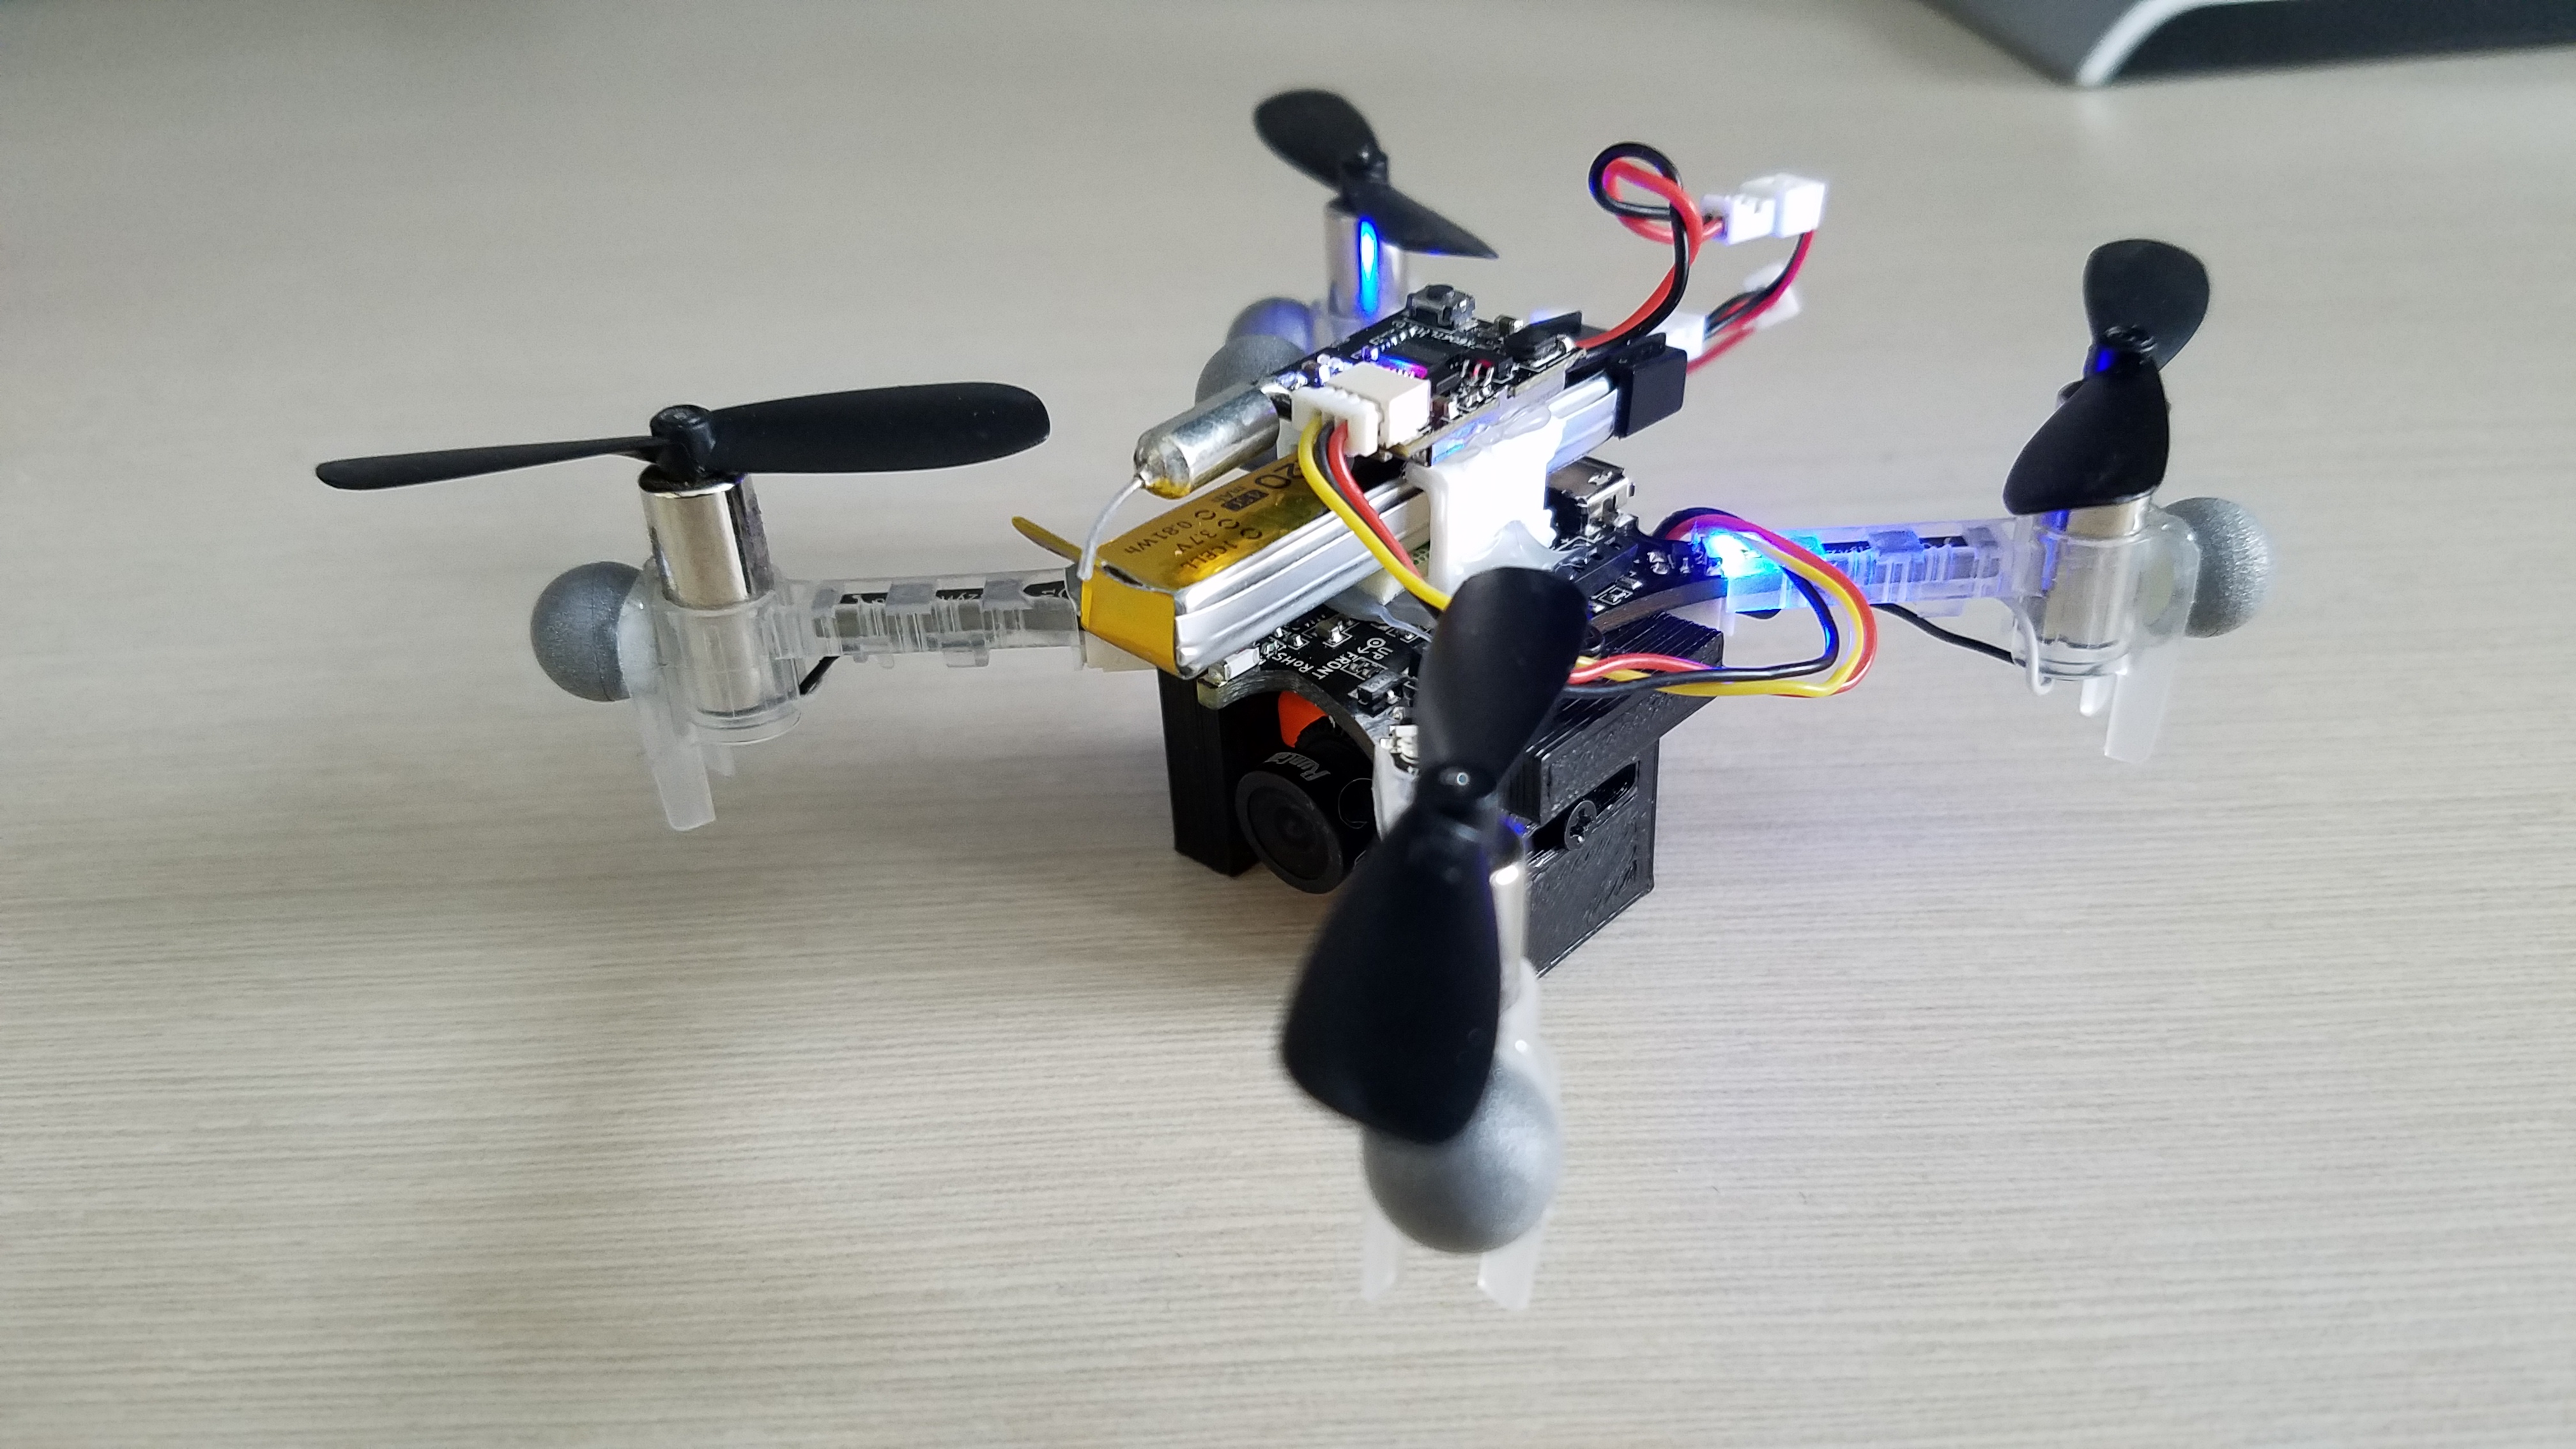
\includegraphics[scale=0.075]{payload1}
    \vspace{10pt}
    \caption[Newly developed UAV payload]{Newly developed UAV payload}
    \label{payload}
\end{figure}

In order to provide ground truth to test against, a motion capture system developed by Vicon is used. By placing lightweight plastic balls in unique configurations on the UAV, the system tracks the full three-dimensional poses of the UAV to an extremely high degree of precision using many cameras. The UAV communicates with the ground station (a basic laptop) through two radio links: a two-way link for UAV commands and basic sensor data streams and a separate link for camera image data to reduce latency on both links.

\begin{figure}
	\centering
	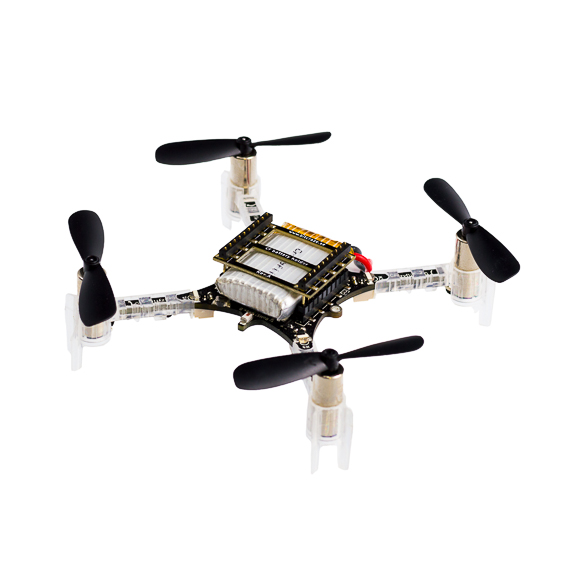
\includegraphics[scale=1.0]{crazyflie_new}
	\caption[The Crazyflie micro-UAV]{The Crazyflie micro-UAV}
	\vspace{8pt}
	\small Source: \url{https://www.bitcraze.io/crazyflie-2/}
	\label{crazyflie_image}
\end{figure}



\begin{figure}
	\centering
	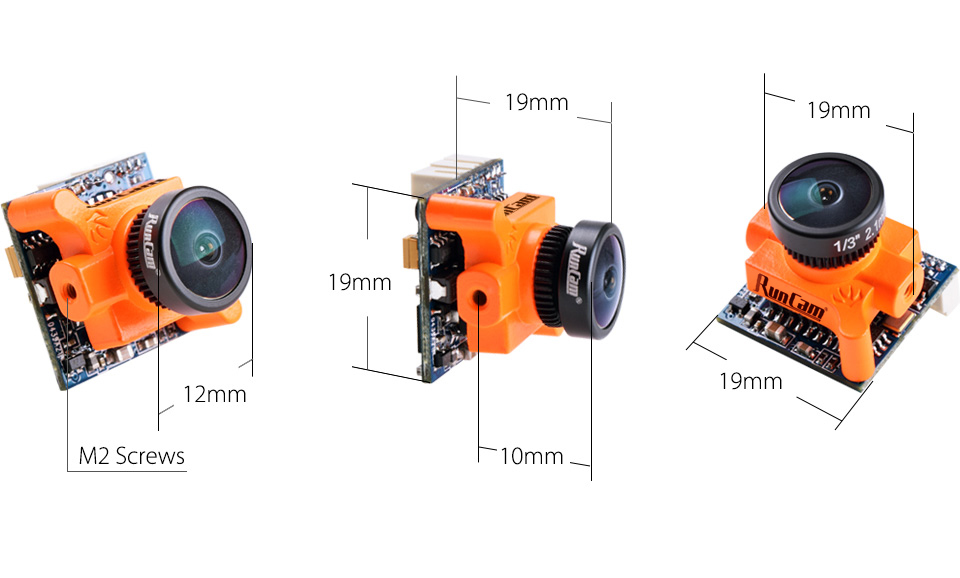
\includegraphics[scale=0.2]{micro-swift-size}
	\caption[The RunCam Micro Swift Camera]{The RunCam Micro Swift Camera}
	\vspace{8pt}
	\small Source: \url{https://shop.runcam.com/runcam-micro-swift/}
	\label{crazyflie_cam}
\end{figure}

In order to control the UAV, the Robotic Operating System (ROS) is used. ROS allows communication between running processes creating greater modularity in code. Processes become ROS nodes which each can handle a different aspect of robotic control. A node for interacting with the Crazyflie, called \verb|crazyflie_ros|\cite{crazyflie_ros}, exists and implements several important features. It allows complete waypoint navigation of the UAV based on PID loops when used with a motion capture system to localize the UAV and generally handles much of the low level UAV control. Without a motion capture system, the node uses the onboard IMU and motor speeds to respond to pitch, roll, yaw, and thrust level commands from other ROS nodes. This node has been tested and functions well in both waypoint and low-level command regimes. 

A software-in-the-loop (SITL) simulation of the task environment has also been set up in the Gazebo robotics simulator based on \verb|sim_cf|\cite{sim_cf}, a firmware simulator for the Crazyflie. Gazebo outputs the same information as the VICON system, if needed, allowing the simulation to closely mimic the control structure of the real world problem. A room with a door has been added to the simulation (Figure \ref{gazebo}), along with a UAV matching the characteristics of the Crazyflie. The ROS interface provided by Gazebo and \verb|sim_cf| is used to send commands in a format identical to what \verb|crazyflie_ros| expects and outputs IMU and camera data in the same format as \verb|crazyflie_ros| does as well. In order to replicate the real-life environment more precisely, the IMU data generated by Gazebo has artificial noise added to it, and the camera similarly has noise added and is lowered in resolution. Both data streams have delays associated with them as well in order to mimic the latency of the data links in real life. 
\begin{figure}
	\centering
	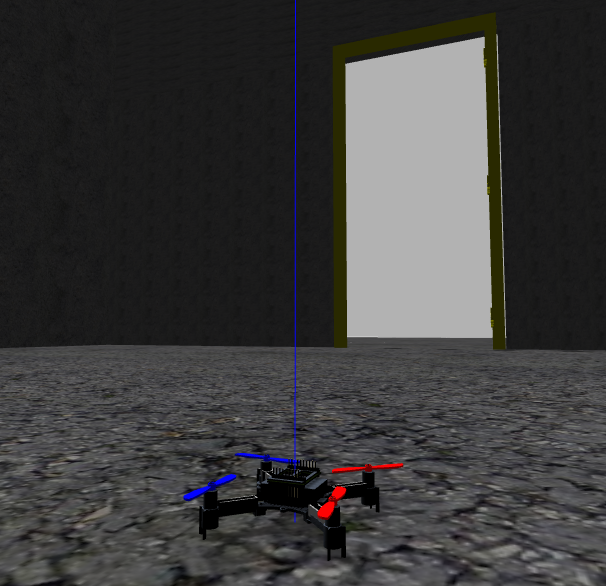
\includegraphics[scale=0.5]{gazebo}
	\vspace{20pt}
	\caption[Simulated Crazyflie Environment]{Simulated Crazyflie Environment}
	\label{gazebo}
\end{figure}

The camera attached to the UAV is forward-facing with the lens pointing out along the UAV's x-axis. The camera-UAV transform has been calibrated for more precise measurements due to the impossibility of perfect camera mounting by a human. Given the assumption of the IMU as the ``center'' of the UAV, which for the Crazyflie is sufficiently close to true, the motion of the camera and the IMU can be correlated to determine how they are related spatially. Correlation has been done with Kalibr\cite{Kalibr}, a calibration toolbox developed by ETH Zurich. The camera itself has also been calibrated using the same package. The \verb|image_undistort| \cite{image_undistort} node, also from ETH Zurich, has been set up to perform undistortion of the images coming from the UAV in real time using the performed calibration. 

\subsection{Image-Based Door Detection}
Software was written which is able to determine where in the UAV's camera image it thinks a door is visible. This software takes an image as input and outputs the $(x,y)$ coordinates it considers to be the middle of the door. Unlike other works, we focus here on getting accurate predictions of the door center, not of a bounding box around the door. This is because the most relevant piece of information to fly through a door is where the center of the door is located. Where the rest of the doorframe is located is not hugely important when the tiny UAV is most likely able to fly through the door as long as it flies through the center. The door must be correctly identified with a high success rate in order to make the entire work successful. It must perform this correct identification in many environments, as the door will not always be placed directly in front of the UAV with a clear distinction between the door and surrounding wall. The door might appear very different due to the UAV's perspective and could be only partially visible during some stages of the UAV's flight, such as when it approaches very close to the door. Door detection was achieved in multiple ways: through a method relying on the Hough transform to find doorframe edges in the image, and through a convolutional neural network.

\subsubsection{Hough Transform-Based Method}
In the Hough-based method the camera image, once received, is converted to grayscale. After bilateral filtering, the edges in the $x$ and $y$ directions of the image are detected using a Canny edge detector. These edges are then thresholded to select only the strongest edges which might be the doorframe. The edges are then converted into the Hough space. To do this, each pixel in the image has several lines associated with it, specifically ones which are firstly perpendicular to rays leaving the image origin and secondly pass through the pixel. A ``vote'' for these associated lines is recorded. The lines with a number of votes above a threshold will be selected as lines in the image. 

Significant filtering of the resulting lines is done to reduce the effects of image noise and multiple detections of the same line. The amount of filtering and line suppression is a key tunable parameter that strongly affects the performance of the algorithm. After suppression, lines which are relatively parallel (within a small angle of each other) are grouped together using a k-means clustering. This results in two groups of lines, one going vertically and the other horizontally. The intersection point of the lines within each group is then calculated and treated as a vanishing point of the image. Since we expect there to be a door in the image this assumption of two vanishing points should hold (one formed by the uprights of the door and the other formed by the crossbar/floor). The vanishing points are used to construct a vanishing line which is used to rectify the image to be fronto-parallel to the camera. The fronto-parallel view is a transformation of the image, so it appears to be taken with the camera on the normal of the plane the door lies in. The door should have a consistent aspect ratio in this view, but some variation does occur. The same transform is used on the detected sets of lines. Rectangles in the transformed set of lines are then generated by grouping sets of parallel/perpendicular lines, and the largest that matches the standard door aspect ratio is selected as the door. The center of this rectangle is output as the result (after inverse transforming it back into the original view). 

Due to noise and motion blur, reasonable vanishing points cannot always be determined. Since the previously described sequence depends on the points to rectify the image and determine the door rectangle, a tracker is introduced to allow a reasonable door center to be output when the image could not be rectified. A Median Flow tracker \cite{medianFlow} was selected for its high-speed yet accurate performance on image streams where the object might be occluded or changing scale. This tracker is re-initialized whenever an image is able to be rectified, and tracks the pixels in the last determined door rectangle otherwise. The Hough Transform approach suffers from the fact that this entire process is lengthy and possibly slow, meaning it struggles to run in real time. Additionally, when the UAV moves very quickly, the tracker is unable to keep up with the door moving so fast in the image and can lose tracking in this way. If a full view of the door is not seen for a little while the tracker is also not re-initialized and loses accuracy over time. 

\subsubsection{Convolutional Neural Network Method}
The second door detection method uses a convolutional neural network (CNN) to determine the center of the door in the image. Several architectures were explored to find the one best suited for this task. The ADE20K scene dataset\cite{csail_data_1} was parsed for images of doors, and those images were manually annotated with bounding boxes on the doors to generate the training and validation datasets. Initially, full segmentation of the door was attempted using the U-Net architecture \cite{Unet}. While this was moderately successful (Figure \ref{Unet_output}), it took several seconds to process per image on the ground station laptop which was far too slow for real-time control of the UAV.

\begin{figure}
	\centering
	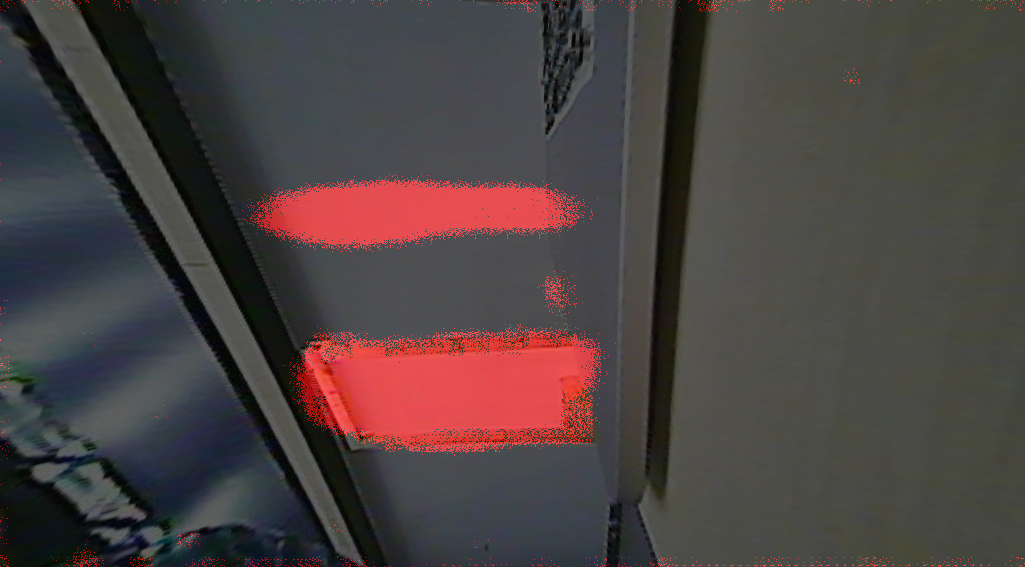
\includegraphics[scale=0.25, angle=270]{Unet_output}
	\vspace{10pt}
    \caption[Result of U-Net Segmentation]{Result of U-Net Segmentation (door pixels are red)}
	\label{Unet_output}
\end{figure}

A custom architecture was also developed for this task. Using the image as input, it passes the image through several convolutional layers (each of which is followed by a max-pooling operation), after which the last layer is fed through a fully-connected layer with two outputs: the $x$ and $y$ coordinates of the door center. This architecture (as seen in Figure \ref{arch}) was chosen due to its small size since it was to run on the UAV ground-station which has limited resources. The number of convolutions learned at each level is much smaller than in related networks such as in \cite{NNDoor}: just 8, then 16, then 32. This also speeds processing of each image. This network was unable to learn to detect the center of a door consistently. 

Tiny-YOLO \cite{yolov3} was selected as a possible architecture due to its small size but high accuracy instance detection results. A standard implementation of the algorithm \cite{keras-yolo3} was modified for detecting doors. After training, it was noted that when an image of a door was taken from a relatively fronto-parallel point, the network would often detect each vertical frame piece of the door as a separate door. This is possibly due to the presence in the training set of images of doors at very oblique angles, making them look like only the upright portion. In order to rectify this, the YOLO loss function (Equation \ref{YOLOloss}) was modified by re-weighting each of the terms. During algorithm runtime, each image is divided into a $7x7$ grid, and detection is performed in each grid cell using standard anchor boxes. The loss function computes the sum over each grid cell of the accuracies of detections in grid cell $i$. If there is a detection ($\mathbbm{1}$), the $x,y$ location of the detection, the width and height ($w,h$) of the detection, and the class confidence ($p_i(c)$) are compared to their ground truth values, and the sum of these comparisons is used as the accuracy of the detection. By weighting the width term to be more significant, the network learned to be more accurate with the width of detections at the cost of slightly lower accuracy in the other metrics. The lower accuracy is acceptable as the width of the bounding box is key to the center of the box being correctly placed over the center of the door. Re-weighting yielded significantly better results like in Figure \ref{yolo_out}, and the trained Tiny-YOLO network is used as the representative of convolutional neural network techniques for comparison with the Hough method. The final output of the standard YOLO network is a set of possible bounding boxes. To convert these to a single door center, the highest confidence detection is selected and the center of the predicted bounding box used as the predicted door center. If no high confidence detections are returned, a Median Flow tracker tracks the pixels in the previous detection.

\begin{equation}
\sum_{i = 0}^{48} \biggl( \lambda \mathlarger{\mathbbm{1}}_i^{\text{obj}}\bigl((x_i - \hat{x}_i)^2 + (y_i - \hat{y}_i)^2 + (\sqrt{w_i} - \sqrt{\hat{w}_i})^2 + (\sqrt{h_i} - \sqrt{\hat{h}_i})^2\bigr) + \sum_{c \in \text{classes}} (p_i(c) - \hat{p}_i(c))^2 \biggr)
\label{YOLOloss}
\end{equation}

\begin{figure}
	\centering
	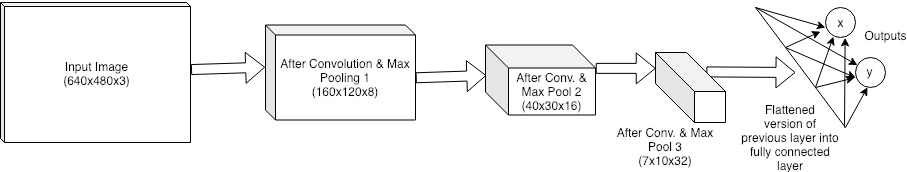
\includegraphics[scale=0.5]{arch}
	\vspace{20pt}
	\caption[Sample door detection network architecture]{Sample door detection network architecture}
	\label{arch}
\end{figure}

\begin{figure}
	\centering
	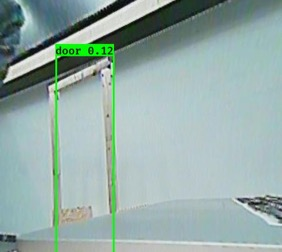
\includegraphics[scale=0.55]{yolo_out}
	\vspace{20pt}
	\caption[Sample YOLO output]{Sample YOLO output}
    \label{yolo_out}
\end{figure}

\subsubsection{Comparison and Results}
The error of a detection can be calculated by the Euclidean distance from the detection $(x,y)_{predicted}$ to the ground truth center of the door $(x,y)_{groundtruth}$. However, this does not take into account the fact that an error of $\epsilon$ is far more significant when the width of the doorframe in the image is approximately $\epsilon$ than if the width is $>>\epsilon$. To take the doorframe size into account, scaled accuracy (closer to zero is better) is defined as: 
\begin{equation}
    ScaledAccuracy = \frac{\sqrt{(x_{predicted}-x_{groundtruth})^2 + (y_{predicted}-y_{groundtruth})^2}}{TrueDoorArea}
\end{equation}

In order to calculate the scaled accuracy and compare the different methods, two test videos were taken of doors with the UAV's camera. The first dataset consisted of a fake plywood door on an uncluttered background. Dataset 1 was intended to be an easy detection task due to the simplicity of the environment. The second dataset contained multiple real doors in a cluttered environment to see how well each method generalizes to a harder case. Each video was hand-annotated with the correct location of the door in each frame. 

The detection results of each method were compared frame by frame with the annotated ground truth and the scaled accuracy computed for each frame in both datasets. Figure \ref{accuracy} shows a histogram of frames with specific scaled accuracy scores. Overall, the CNN method outperforms the Hough method in both datasets, with the center of the scaled accuracy score distribution lower for the CNN method. An artifact of Dataset 2 is seen in the accuracy scores for the Hough method. The Hough method often failed entirely to detect or track anything in Dataset 2. The default detection for this method, if everything else fails, is to predict the center of the image as the door. Dataset 2 sweeps past the centers of the doors fairly often, meaning that at least some number of detections received very low scaled accuracy scores. These falsely accurate detections lead to the tall column of low scaled accuracy scores followed by a big drop seen by the Hough method on Dataset 2.

\begin{figure}
\centering
\begin{subfigure}{.5\textwidth}
  \centering
  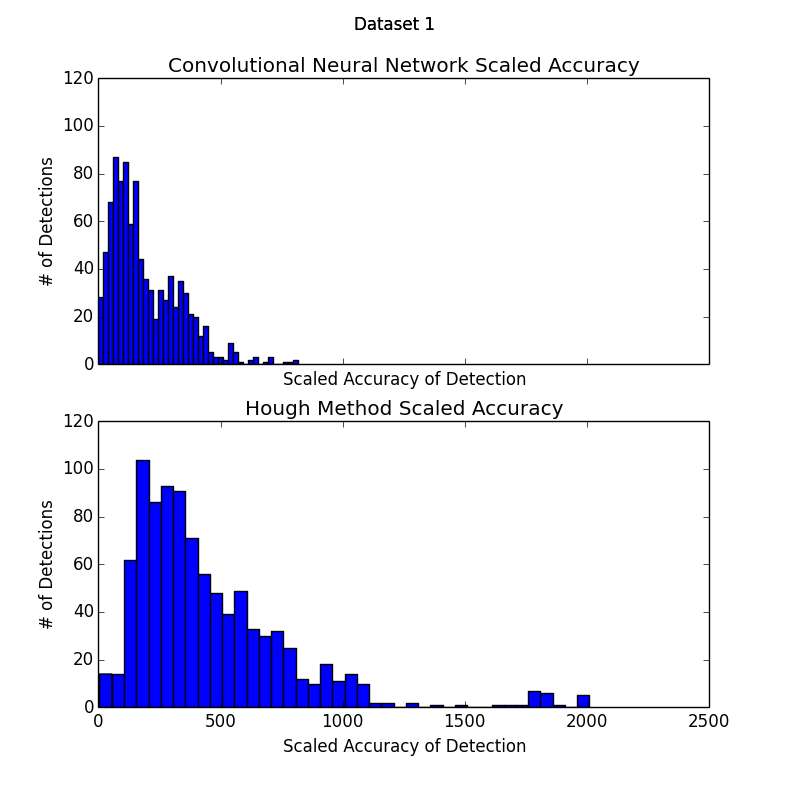
\includegraphics[width=1.1\textwidth]{AccuracyComparison1}
  \caption{Dataset 1}
  \label{Dataset1}
\end{subfigure}%
\begin{subfigure}{.5\textwidth}
  \centering
  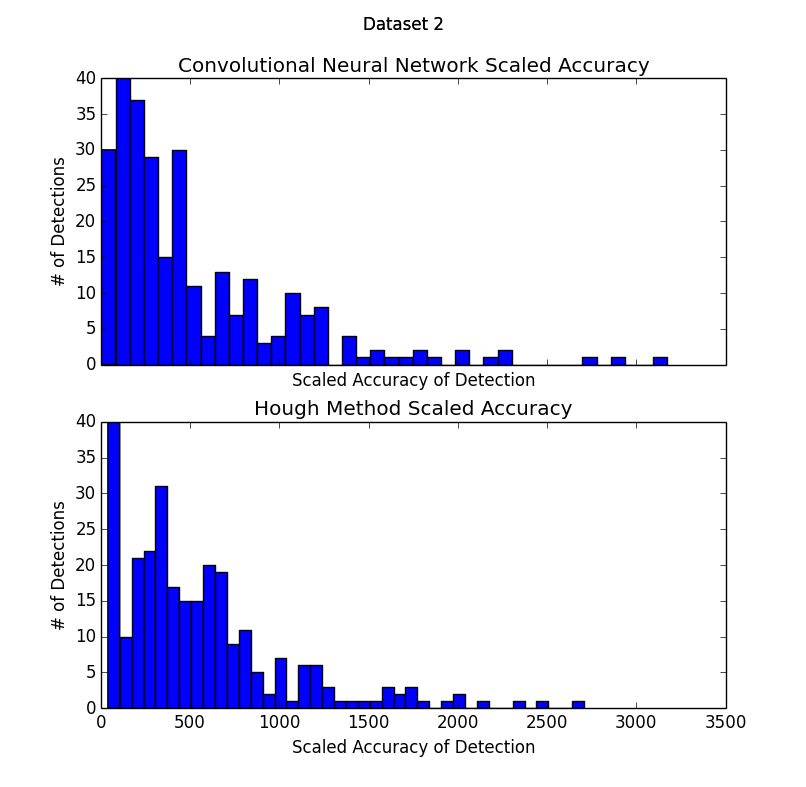
\includegraphics[width=1.1\textwidth]{AccuracyComparison2}
  \caption{Dataset 2}
  \label{Dataset2}
\end{subfigure}
\vspace{20pt}
\caption[Scaled accuracy of Hough and CNN methods on two datasets]{Scaled accuracy of Hough and CNN methods on two datasets}
\label{accuracy}
\end{figure}


In addition to error rate, the speed of the method is a key factor. The UAV provides images at about 30 frames per second (fps), and previous experience suggests that a control loop for the UAV must run at at least 10 Hz. The best method must thus also be able to run ideally at faster than 10 Hz, in order to process each frame and give some time for the control loop code to run so it can achieve 10 Hz. The timing results for both methods are shown in Tables \ref{timing1} and \ref{timing2} as the average time to return a detection. The CNN again outperforms the Hough method and is far more consistent (lower standard deviation across all timings). A similar artifact is seen in these results as before, where it seems as though the Hough method performs much better on Dataset 2 over Dataset 1. This is again because the method failed to detect anything. With very few lines detected, the method is not able to rectify the image and compute a prediction, so it just returns the default prediction early and quickly. Something somewhat similar happened to the CNN on Dataset 2 since much fewer detections were returned for each image. This meant that the post-processing of removing low confidence detections occurred more quickly. In addition, more frames were tracked as opposed to detected by the CNN method in Dataset 2, meaning that the slow action of re-initializing the tracker had to be done less often. 

\begin{table}[H]
\begin{tabular}{l|l|l|}
\cline{2-3}
                                          & Hough Method & Convolutional Neural Network \\ \hline
\multicolumn{1}{|l|}{Mean sec/image}      & 1.11         & 0.89                         \\ \hline
\multicolumn{1}{|l|}{Std. dev. sec/image} & 1.99         & 0.024                        \\ \hline
\end{tabular}
\vspace{20pt}
\caption{Timing Results Dataset 1}
\label{timing1}
\end{table}

\begin{table}[H]
    \begin{tabular}{l|l|l|}
\cline{2-3}
                                          & Hough Method & Convolutional Neural Network \\ \hline
\multicolumn{1}{|l|}{Mean sec/image}      & 0.08         & 0.072                        \\ \hline
\multicolumn{1}{|l|}{Std. dev. sec/image} & 0.02         & 0.009                        \\ \hline
\end{tabular}
\vspace{20pt}
\caption{Timing Results Dataset 2}
\label{timing2}
\end{table}

Overall, it appears the CNN-based method for detecting a door in an image is more successful, consistent, and faster than the Hough method. Depending on the specific dataset, it could meet the 10 Hz requirement and simply needs a more powerful ground station to run more quickly. A possible failing of the Hough method is its high number of tunable parameters. The suppression factor for detected lines, the threshold of pixels for the Hough transform to consider something a line, the aspect ratio range candidates must fall into, and more are all tunable parameters and affect the performance of the Hough method on a specific dataset. The Hough method was tuned on Dataset 1 and thus performed somewhat better than on Dataset 2, indicating the method's difficulty in generalizing.

\subsection{Independent Flight}
The final portion of this work removes the motion capture system from the equation, requiring the UAV to fly without outside knowledge of its orientation and location. In place of the motion capture system, the onboard IMU and camera are used to both keep the UAV stable and provide information about how the UAV is currently flying. A series of pitch, roll, yaw, and thrust commands are generated constantly by the selected control algorithm. Two different systems were developed and tested to see their effectiveness at successfully flying the UAV through the door. The first is a classical proportional-derivative (PD) controller, with the error being the difference between the predicted center of the door and the UAV's heading. The second is a recurrent neural network (RNN) which uses the IMU output, the camera image, and the detected center of the door as input to output a stream of commands after having been trained to mimic test flights. 

\subsubsection{PD Controller}
The first approach uses a fairly standard PD controller to minimize the error in the UAV's heading throughout a flight. Given the assumption that the UAV is able to see the door, setting the desired pitch of the UAV to a constant value causes the UAV to move forward, getting closer to the door plane. In order to guarantee that the UAV makes it through, instead of just getting closer to the wall the door is built into, the roll of the UAV (controls left/right movement) is controlled by the image x-axis distance between the predicted door center and the center of the image. Since the camera points straight out from the front of the UAV, minimizing this distance aligns the UAV with a path that leads through the center of the door, causing the constant pitch to carry the UAV through. Thrust (i.e. height of the UAV) is controlled similarly: the distance along the image y-axis between the image center and the predicted door center needs to be minimized to make sure the UAV does not hit the ground or the wall above the door.

In order to minimize these errors, PD control sets the control signal affecting the error to a scaled version of the error (proportional) added to a scaled version of the derivative of the error over time (derivative):
\begin{equation}
Command = K_{p}*Error + K_{d} * \frac{dError}{dt}
\label{PD}
\end{equation}
Proportional control alone led to oscillations around the desired zero error as the method tried to correct, so $K_d$ is tuned to cause the UAV to slow down as it approaches zero error, acting like a spring damper. Equation \ref{PD} was implemented for both thrust and roll. $K_p$ and $K_d$ along with the static pitch angle were tuned using test flights from a selected `zero' location until the UAV made it through the door with minimal oscillation.

\subsubsection{Recurrent Neural Network}
The second approach uses a recurrent neural network (RNN) trained to navigate through the door. An RNN was selected for this task since it has memory, allowing it to handle time dependent quantities like velocities and momentums during flight. Using the motion capture-based waypoint navigation algorithm in \verb|crazflie_ros|, the UAV was flown repeatedly in simulation from the zero location previously mentioned through the door. The RNN trained based on the IMU, camera, and control data generated during these flights. The camera, IMU, door detection, and time are used as inputs to the network, and the network learns to mimic the control data the waypoint navigation algorithm generated at that point. The architecture created for this task involved a small convolutional section to process the image data, which was then flattened and fed alongside the other sensor data to the rest of the network. The rest of the network consisted of several fully connected layers, several Gated Recurrent Unit layers, and a final fully connected layer to generate the actual control outputs. Input and output data was normalized to be zero mean, unit standard deviation to speed training. The normalization factors were saved and used to denormalize the network output at testing time. The full network structure that led to the lowest training error is seen in Figure \ref{rnn_structure}.

\begin{figure}
	\centering
    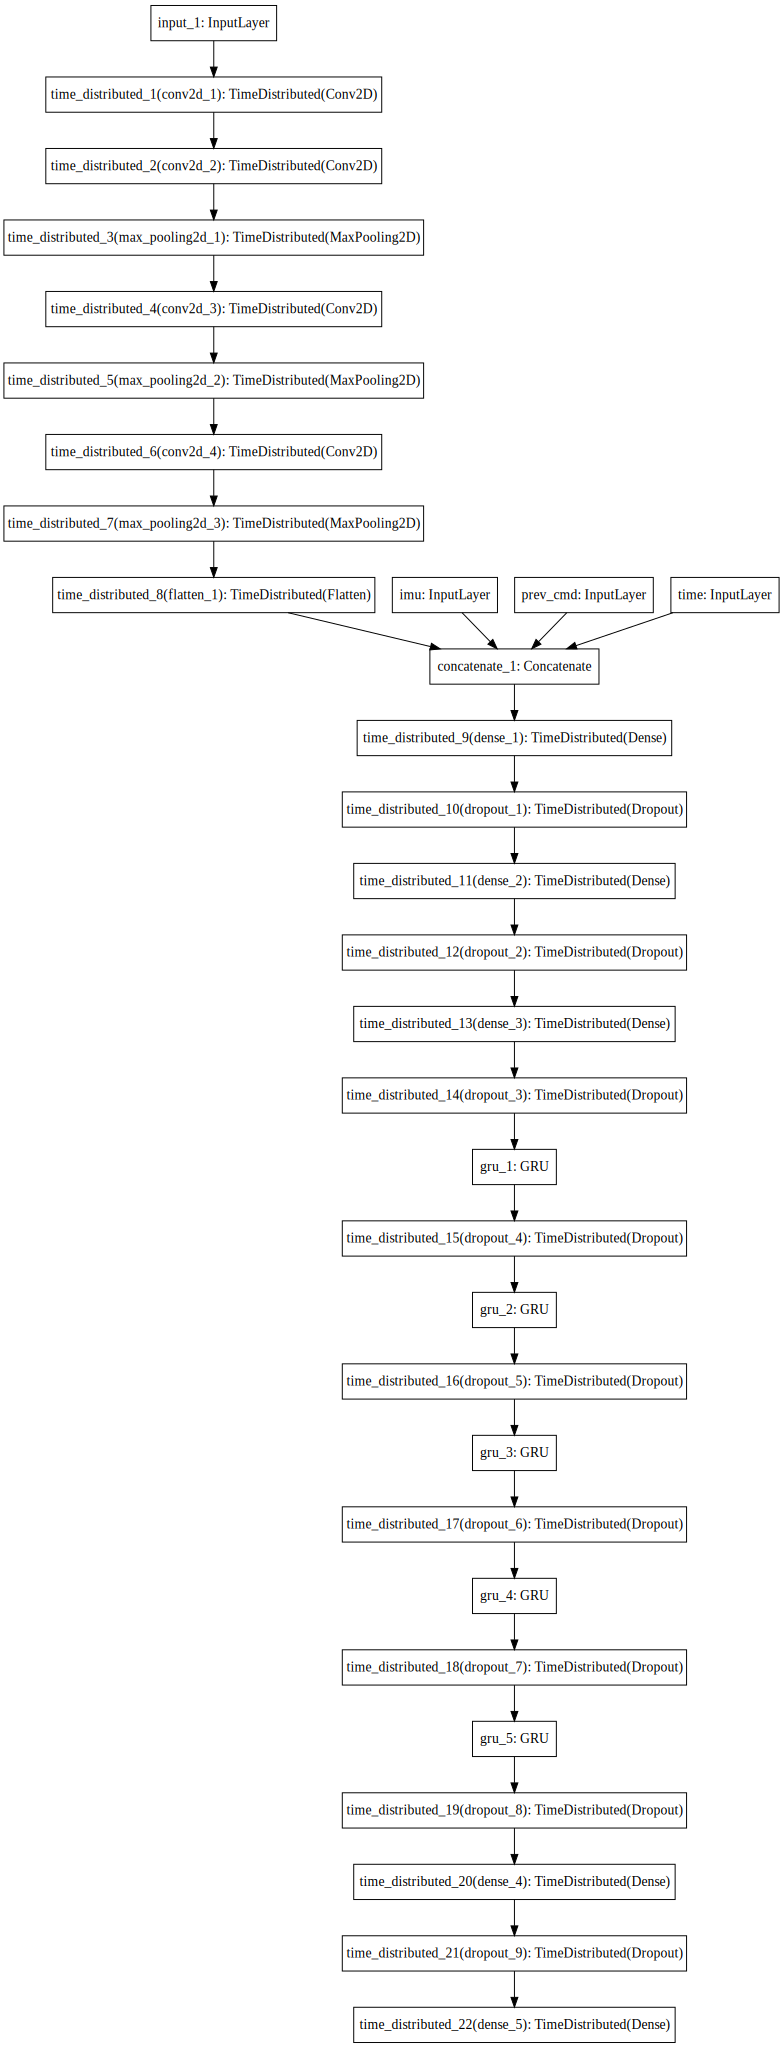
\includegraphics[scale=0.07]{model}
	\vspace{20pt}
	\caption[Recurrent Neural Network Structure]{Recurrent Neural Network Structure}
    \label{rnn_structure}
\end{figure}
\subsubsection{Comparison and Results}
In order to compare the two methods, each was set up to control the UAV through 40 total test flights in simulation. 20 of these flights were done from the zero location where the PD controller was tuned and the RNN training data was collected from. 20 of these flights were started from random locations in the simulated room, taken from a uniform distribution over the area of the room. Table \ref{flight} lists some characteristics of these flights.


\begin{figure}
	\centering
    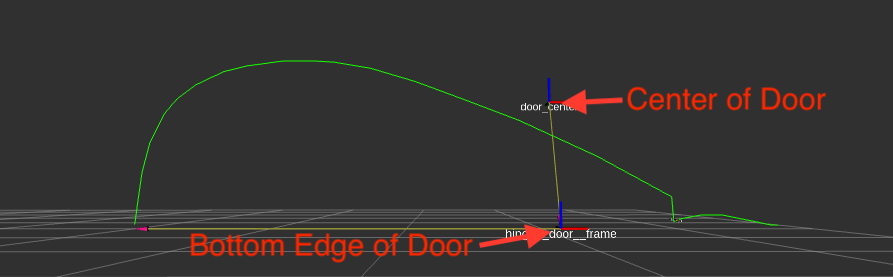
\includegraphics[scale=0.4]{rviz_from_side}
	\vspace{10pt}
	\caption[Successful Flight Path Viewed from Side]{Successful Flight Path Viewed from Side}
    \label{rviz_from_side}
\end{figure}
\begin{figure}
	\centering
    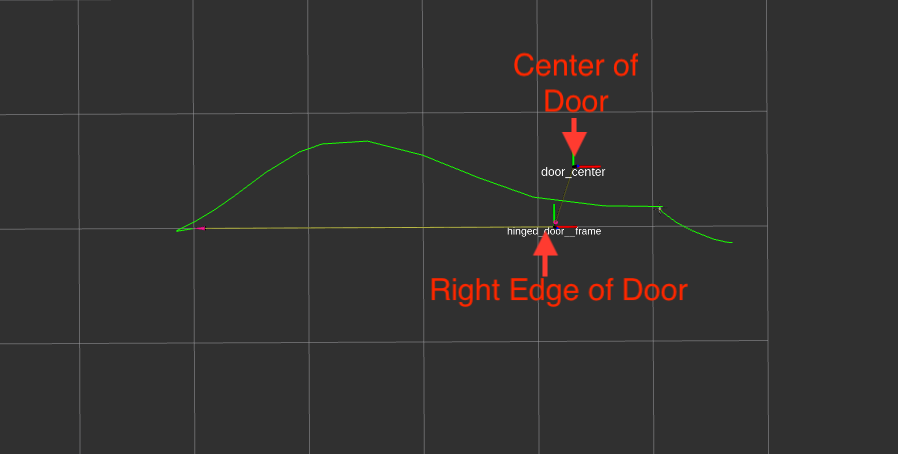
\includegraphics[scale=0.4]{rviz_top_down}
	\vspace{10pt}
	\caption[Successful Flight Path Viewed From Above]{Successful Flight Path Viewed From Top}
    \label{rviz_top_down}
    %\vspace{20pt}
\end{figure}


\begin{table}[]
\begin{tabular}{l|l|l|}
\cline{2-3}
                                                           & PD Control   & RNN Control            \\ \hline
\multicolumn{1}{|l|}{Stable Flight}                        & Yes          & Yes                    \\ \hline
\multicolumn{1}{|l|}{Success rate from zero location}      & 65\% (13/20) & Loops w/o finding door \\ \hline
\multicolumn{1}{|l|}{Success rate from arbitrary location} & 25\% (5/20)  & Loops w/o finding door \\ \hline
\end{tabular}
\vspace{20pt}
\caption{Test Flight Success Statistics}
\label{flight}
\end{table}

A successful flight is defined as making it through the door without bumping/crashing into walls or the edges of the doorframe (Figures \ref{rviz_from_side},\ref{rviz_top_down}). Table \ref{flight} shows the PD controller is the obviously more successful of the two flight controllers. While both were able to make the UAV fly stably (not flip over, crash into the floor, etc), the RNN controller did not show intention of moving towards the door. The stable flight indicates that the network did learn the bounds of reasonable control inputs to the UAV but did not learn the higher level task. It is possible this is due to a noisy dataset; the ground truth waypoint navigation algorithm, while very consistent in getting the UAV through the door often responds to similar perturbations slightly differently each time since the UAV is a complex system. The network was unable to generalize these different reactions and was thus unable to learn to control the UAV to complete its task. The PD controller, on the other hand, was more successful. From the location it was tuned from, it was able to get through the door the majority of the time. From an arbitrary location, the success rate dropped significantly. Additional tuning did not particularly help, yielding unbounded oscillations and crashes into the walls next to the doorframe. While not necessarily the most likely outcome, the PD controller is able to occasionally get the UAV through the door safely. 

In general, neither method was very successful at flying the UAV from an arbitrary location in a room through the door. However, the PD controller's limited successes indicate that there is enough information available to a controller from just the detection and the IMU data to complete the task. Thus, a more complex controller like one that models the Crazyflie's dynamics or a neural network with a different structure or type of layer could possibly learn the function needed to consistently fly the UAV through the door.


%j) Conclusion/Summary – A succinct summary of your proposed project.
\section{Conclusion}
In conclusion, this project explores the applicability of various techniques and approaches to indoor navigation by very small UAVs. To do this, a specific problem is defined: navigating from an arbitrary initial position through a doorway. The sensing package defined is purposely limited to low-cost, low-quality, and relatively high-latency sensors on an extremely small platform in order to explore how navigation and motion might be controlled in sensor-limited environments. To this end, a Crazyflie micro-UAV with a low-resolution camera is selected as the platform for experiments. To complete the task, several discrete pieces of software were written and connected through the Robotic Operating System. 

The first is a door-detection algorithm. Several options for this algorithm were explored including a Hough transform-based algorithm and a convolutional neural network. The network proved to be the more successful of the two methods in both accuracy and speed on novel datasets collected with the real UAV camera. 

Next, a way to navigate through the door without any external localization systems was written. Several options for flight control were developed and tested against one another, including a classical PD controller and a recurrent neural network. A full software-in-the-loop simulation was set up to mimic the real flight of the UAV in order to test the flight controllers. The PD controller proved to be moderately successful and able to fly the UAV through the door from select locations. The recurrent neural network was able to stabilize the UAV but was unable to learn the high level task of getting to the door. 

These results form a basis for further exploration of complex tasks using very small platforms with limited sensing. Task-specific as opposed to general solutions may be necessary due to these constraints, and certain assumptions may need to be made. However, given some problem-specific knowledge, task controllers can be devised to yield results even under severe limitations. 
%k) List of References - Numbered list of references that must include for each reference: authors, title,
%name of the source (e.g. conference, journal, etc.), and date of the publication. You should use the
%citation format that is standard for the primary journals in your specific field of research.
\bibliographystyle{plain}
\bibliography{../../references}

%Written project proposals are typically about 10 to 12 double-spaced pages in length for the main text
%and figures, but excluding the title page, abstract, table of contents, list of figures, budget, timeline, and
%references. They should be in 12-point font with one-inch margins. Introduction(1) + Background(1.5) + Proposed Project(7) + Conclusion(1) is 10-12 pages


%The oral project proposal presentation will give you the opportunity to describe your ideas and to show
%the soundness of your proposed approach to your peers, your project advisor, and the course coordinator.
%This presentation should include all of the above components. Your project proposal presentation should
%be 10 to 12 minutes long, followed by 3 minutes for Q&A.
\end{document}
